\section{Experiments and Results}

All our experiments have been completed with the inexpensive consumer
drone, Parrot's AR Drone 2.0. We have used ROS based ARDrone Autonomy Driver
to communicate with drone. For the purposes of establishing the ground truth,
pictures were taken with a smartphone camera (5 mega pixel) .

We have implemented our algorithm in C++ using the OpenCV library (OpenCV
2.4.9). Experiments were performed on a PC with Intel Core i7 processor(@3.4GHz)
and 8GB RAM. Source code to select images and generate super panorama, as well as the
data sets used in this paper will be made publicly available.


\subsection{Establishing Correctness}

In our first experiment, we wanted to ensure that the selection of
images done was comprehensive.  This experiment was conducted in an
outdoor environment. We note here that there were approximately 9000 images in
the raw video.  Autostitch was unable to cope when fed with these number of images.  
Figure \ref{fig:uniformsampled_sac3} shows uniformly
time sampled images from complete video. Figure \ref{fig:selected_sac3}  shows
examples of selected images. (The video will be made available in the
supplementary material.) Though most of the images are same in both (time
sampled versus selected by our algorithm), there is still some redundancy
(column 1 and column 2 in Figure \ref{fig:uniformsampled_sac3}) in time sampled
images.

\begin{figure*}[htb!]
\centering
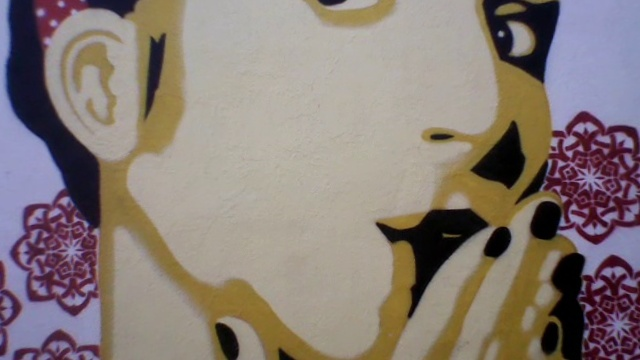
\includegraphics[width=0.19\linewidth]{figures/sac3/uniform_sampled/1.jpg}
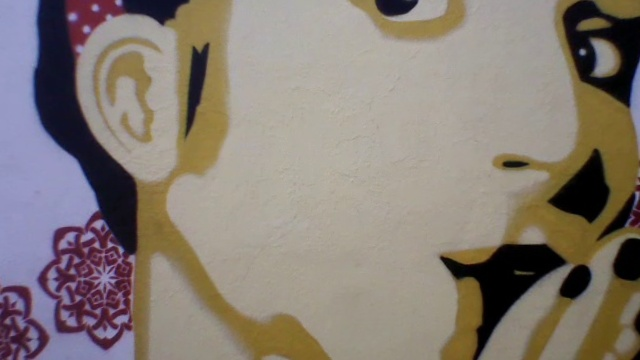
\includegraphics[width=0.19\linewidth]{figures/sac3/uniform_sampled/5.jpg}
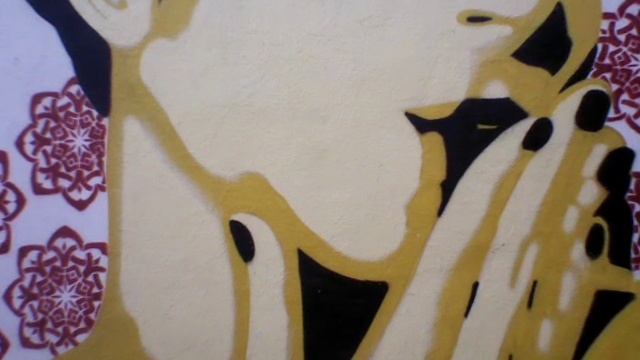
\includegraphics[width=0.19\linewidth]{figures/sac3/uniform_sampled/4.jpg}
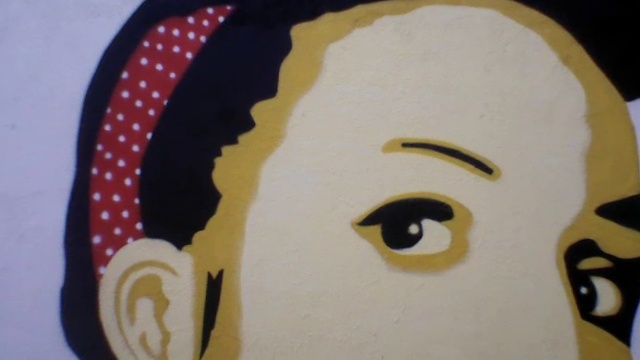
\includegraphics[width=0.19\linewidth]{figures/sac3/uniform_sampled/2.jpg}
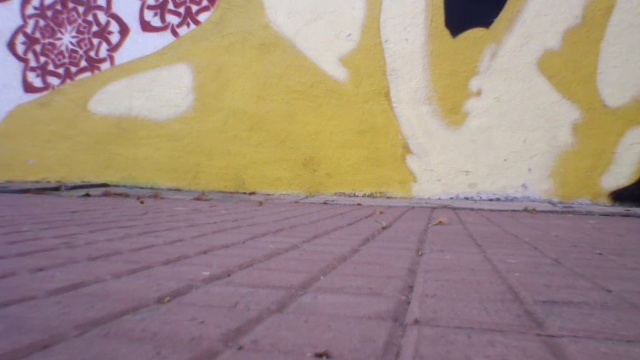
\includegraphics[width=0.19\linewidth]{figures/sac3/uniform_sampled/3.jpg}
\caption{Uniformly time sampled images from whole dataset}
\label{fig:uniformsampled_sac3}
\end{figure*}

\begin{figure*}[htb!]
\centering
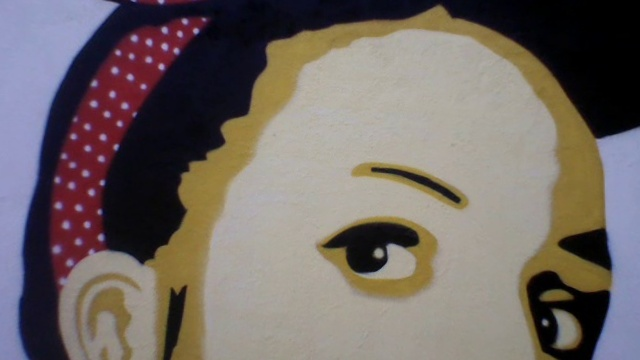
\includegraphics[width=0.19\linewidth]{figures/sac3/selected/1.jpg}
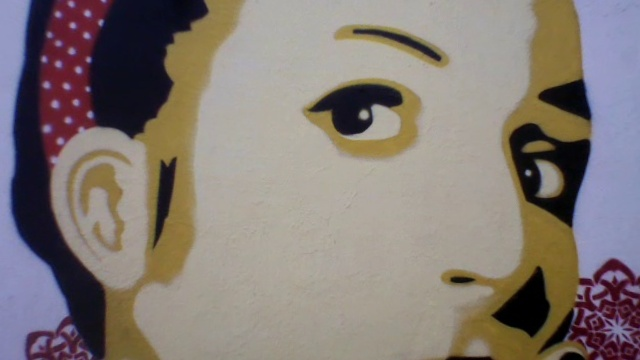
\includegraphics[width=0.19\linewidth]{figures/sac3/selected/5.jpg}
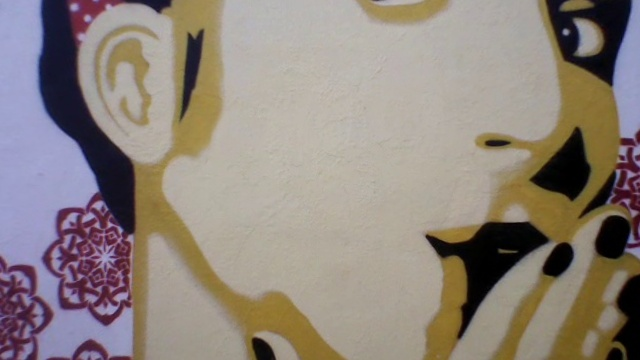
\includegraphics[width=0.19\linewidth]{figures/sac3/selected/4.jpg}
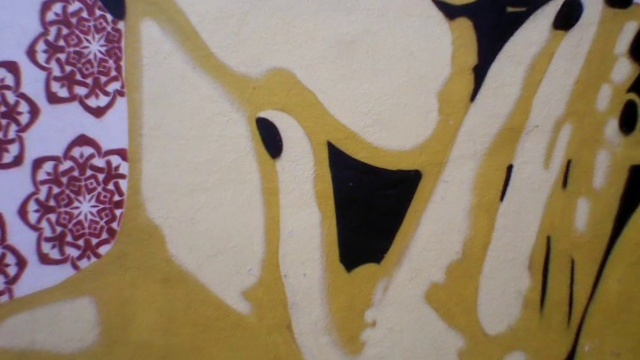
\includegraphics[width=0.19\linewidth]{figures/sac3/selected/2.jpg}
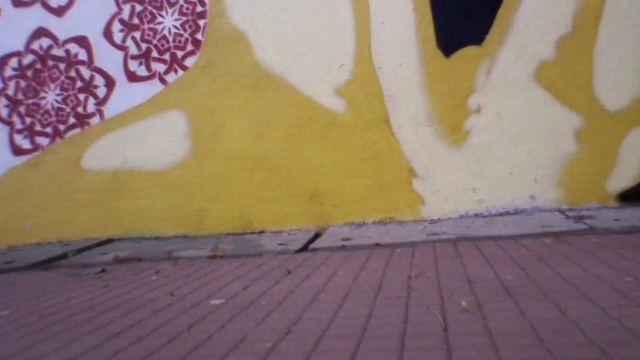
\includegraphics[width=0.19\linewidth]{figures/sac3/selected/3.jpg}
\caption{Sample images selected from the set of approximately 9000 images by our
algorithm using positional information}
\label{fig:selected_sac3}
\end{figure*}

Also, when time sampled images are given to even State of the Art photo stitcher
such as Adobe Photoshop, it could not completely stitch the scene as seen in
Figure \ref{fig:results_sac3_timesmapled}.

\begin{figure*}[t!]
\centering
\begin{subfigure}[b]{0.4\textwidth}
\centering
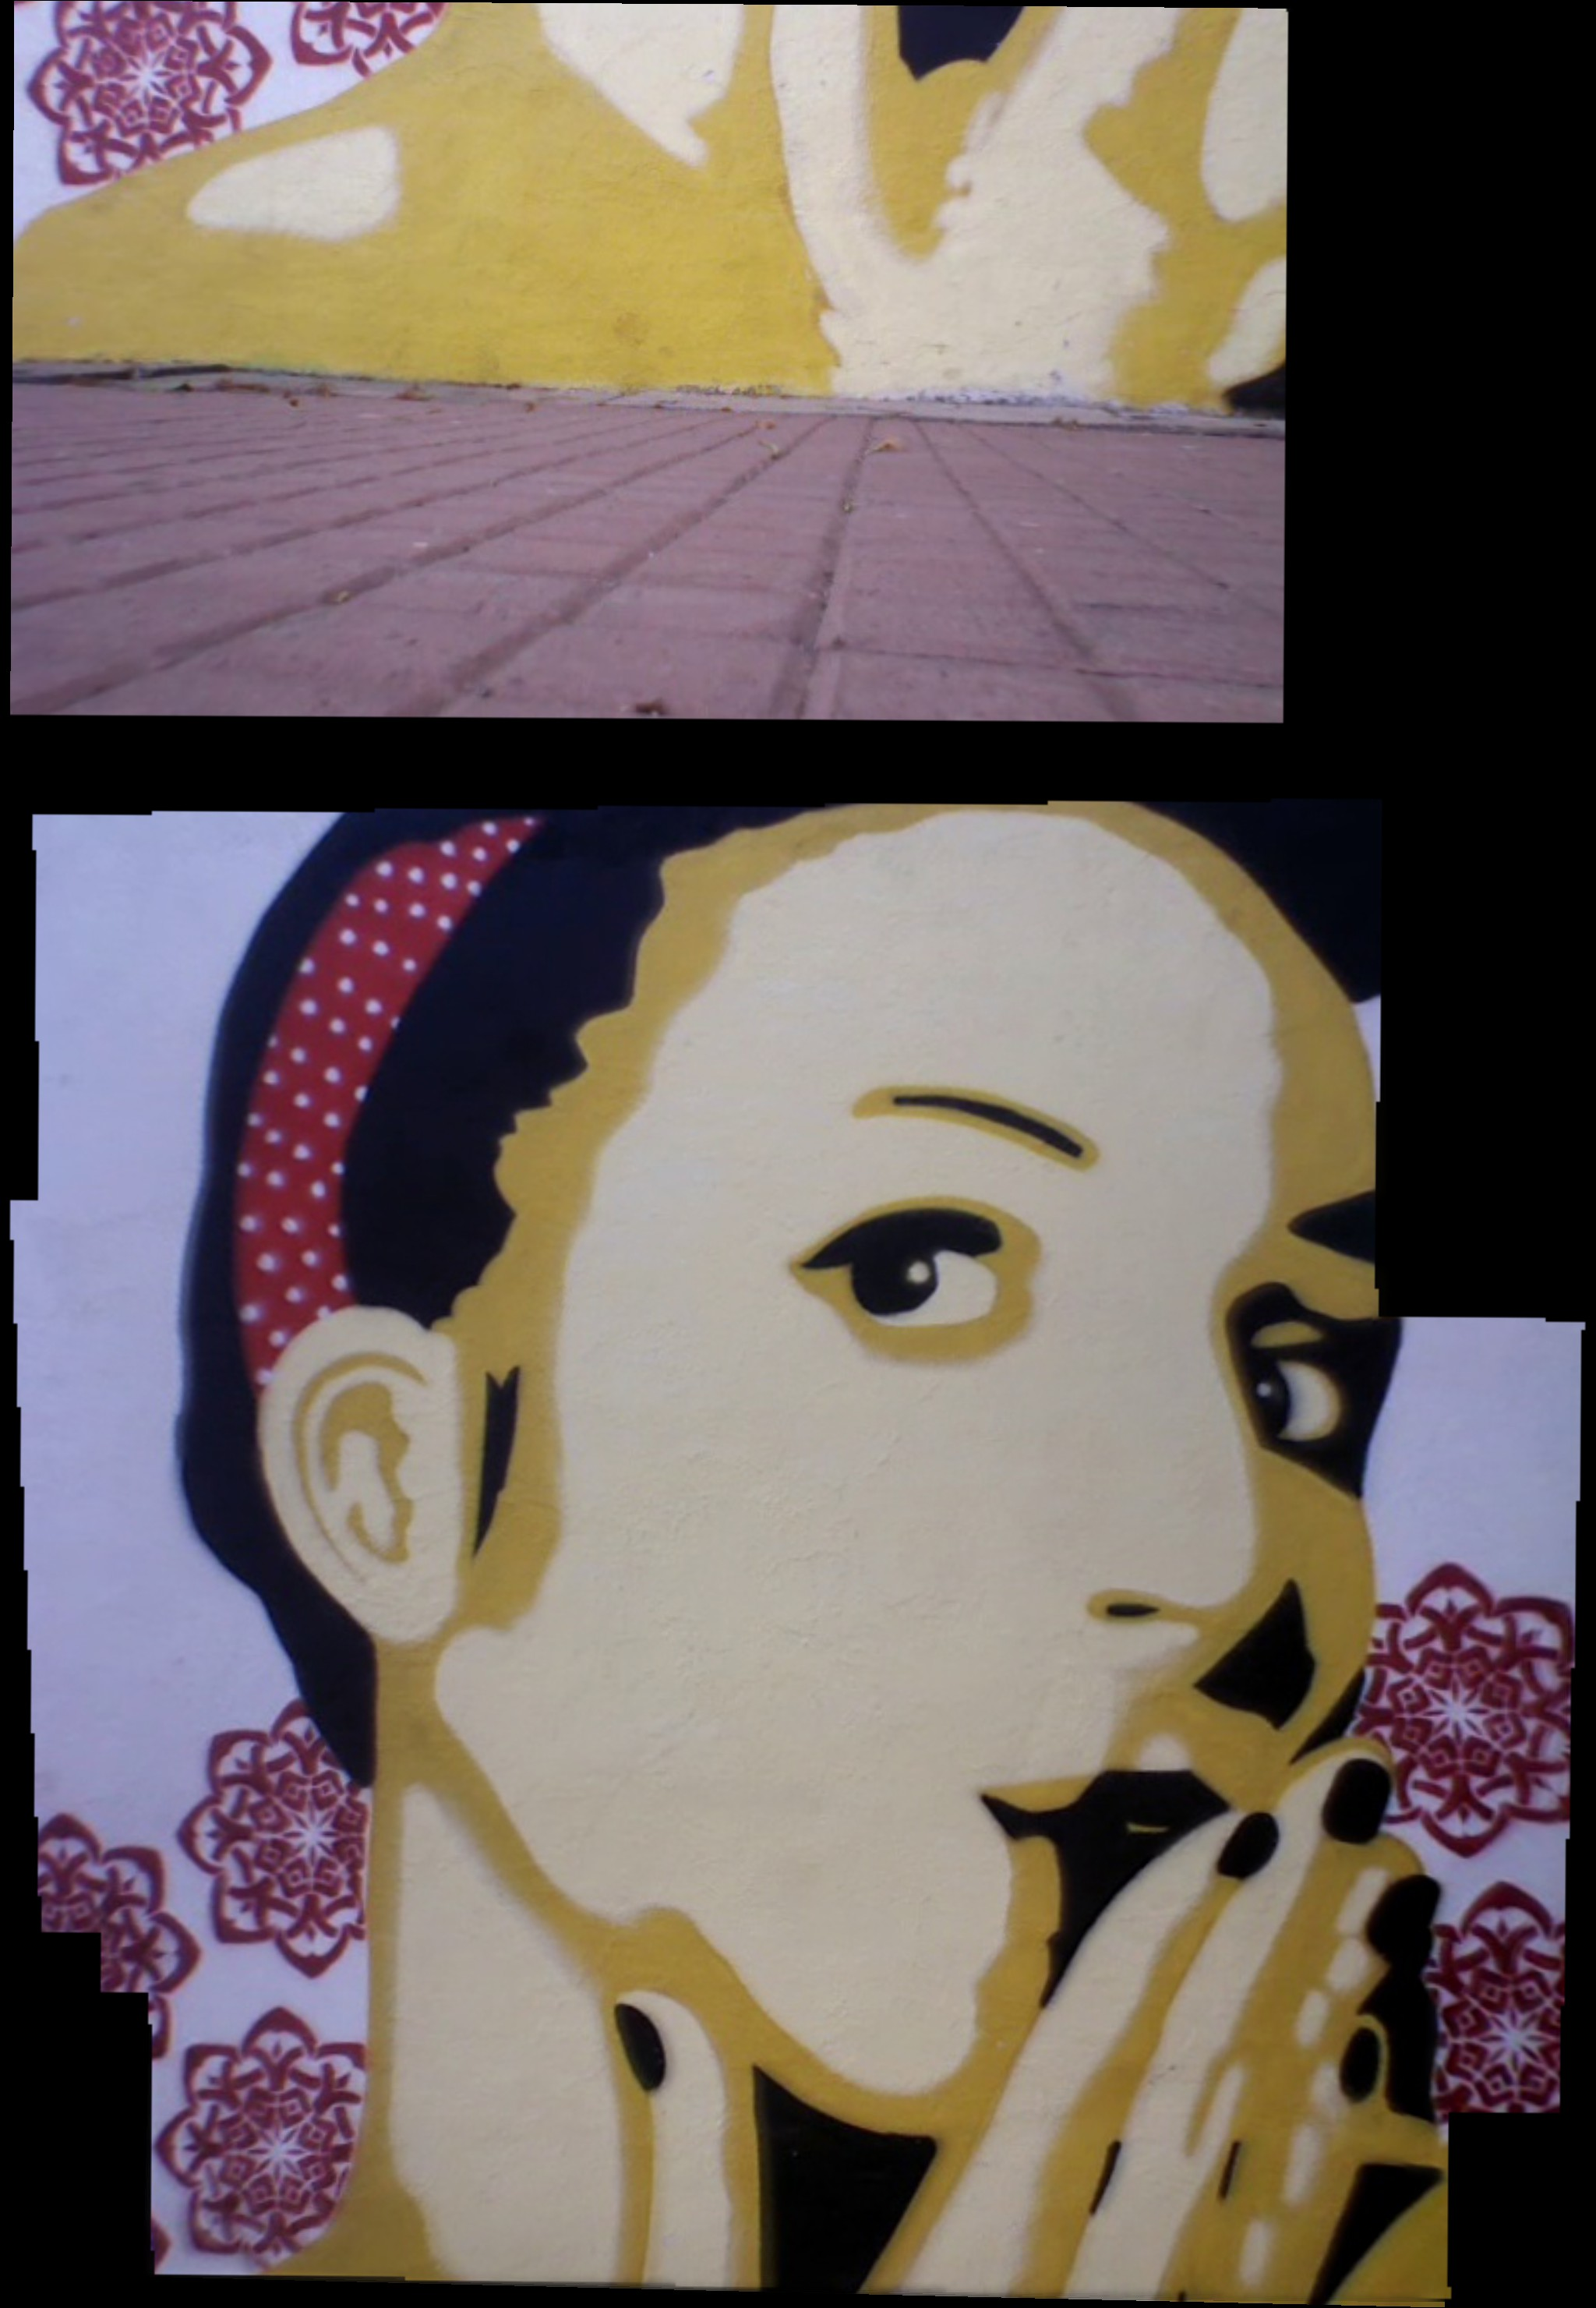
\includegraphics[width=\linewidth]{figures/sac3/uniform_sampled/autostitch.jpg}
\caption{Autostitch Result}
\end{subfigure}
\begin{subfigure}[b]{0.4\textwidth}
\centering
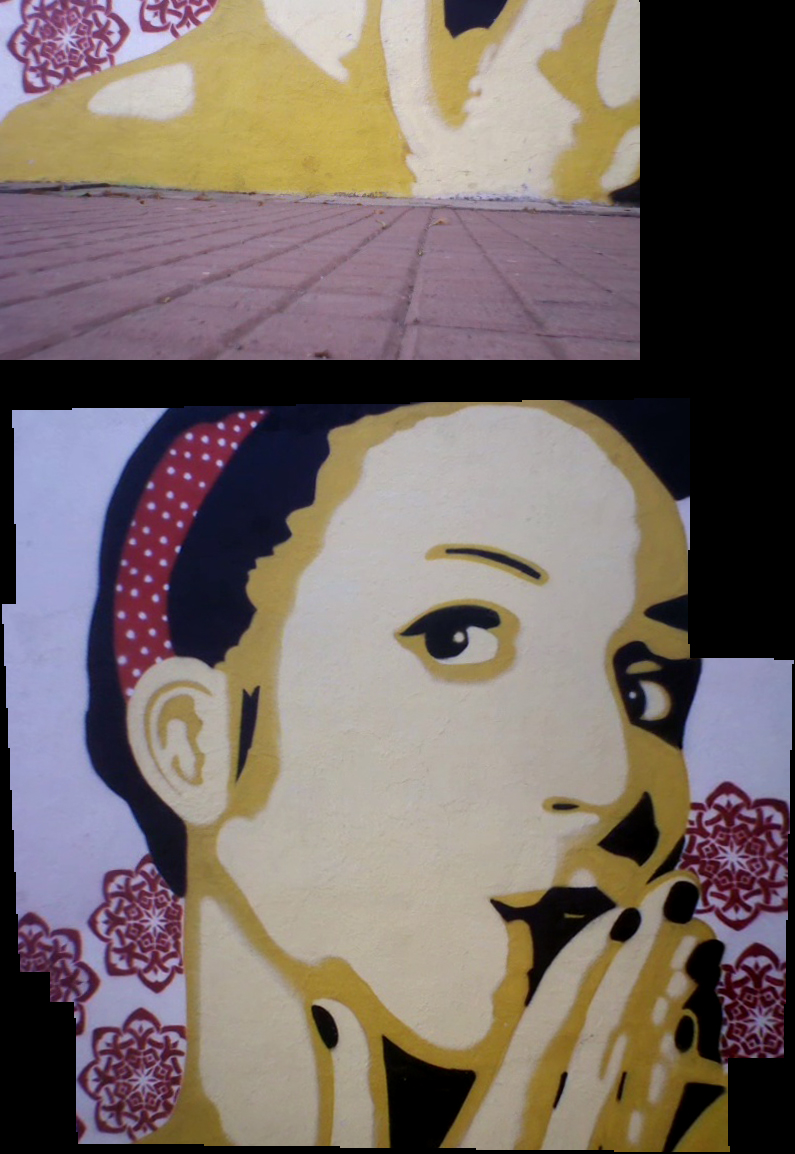
\includegraphics[width=\linewidth]{figures/sac3/uniform_sampled/photoshop.jpg}
\caption{Photoshop Result}
\end{subfigure}
\caption{Output of state of the art photo stitchers on uniformly time sampled
images. As time sampled images doesn't gurantee complete spacewise coverage of
scene, we get broken panorama.}
\label{fig:results_sac3_timesmapled}
\end{figure*}

Our selection algorithm was employed and approximately N=5 images
were obtained. We have given images selected by our algorithm to photo stichers
as well as our stitching code whose outputs can be seen in Figure
\ref{fig:results_sac3_timesmapled}.
 
\begin{figure*}
\centering
\begin{subfigure}[b]{0.3\textwidth}
\centering
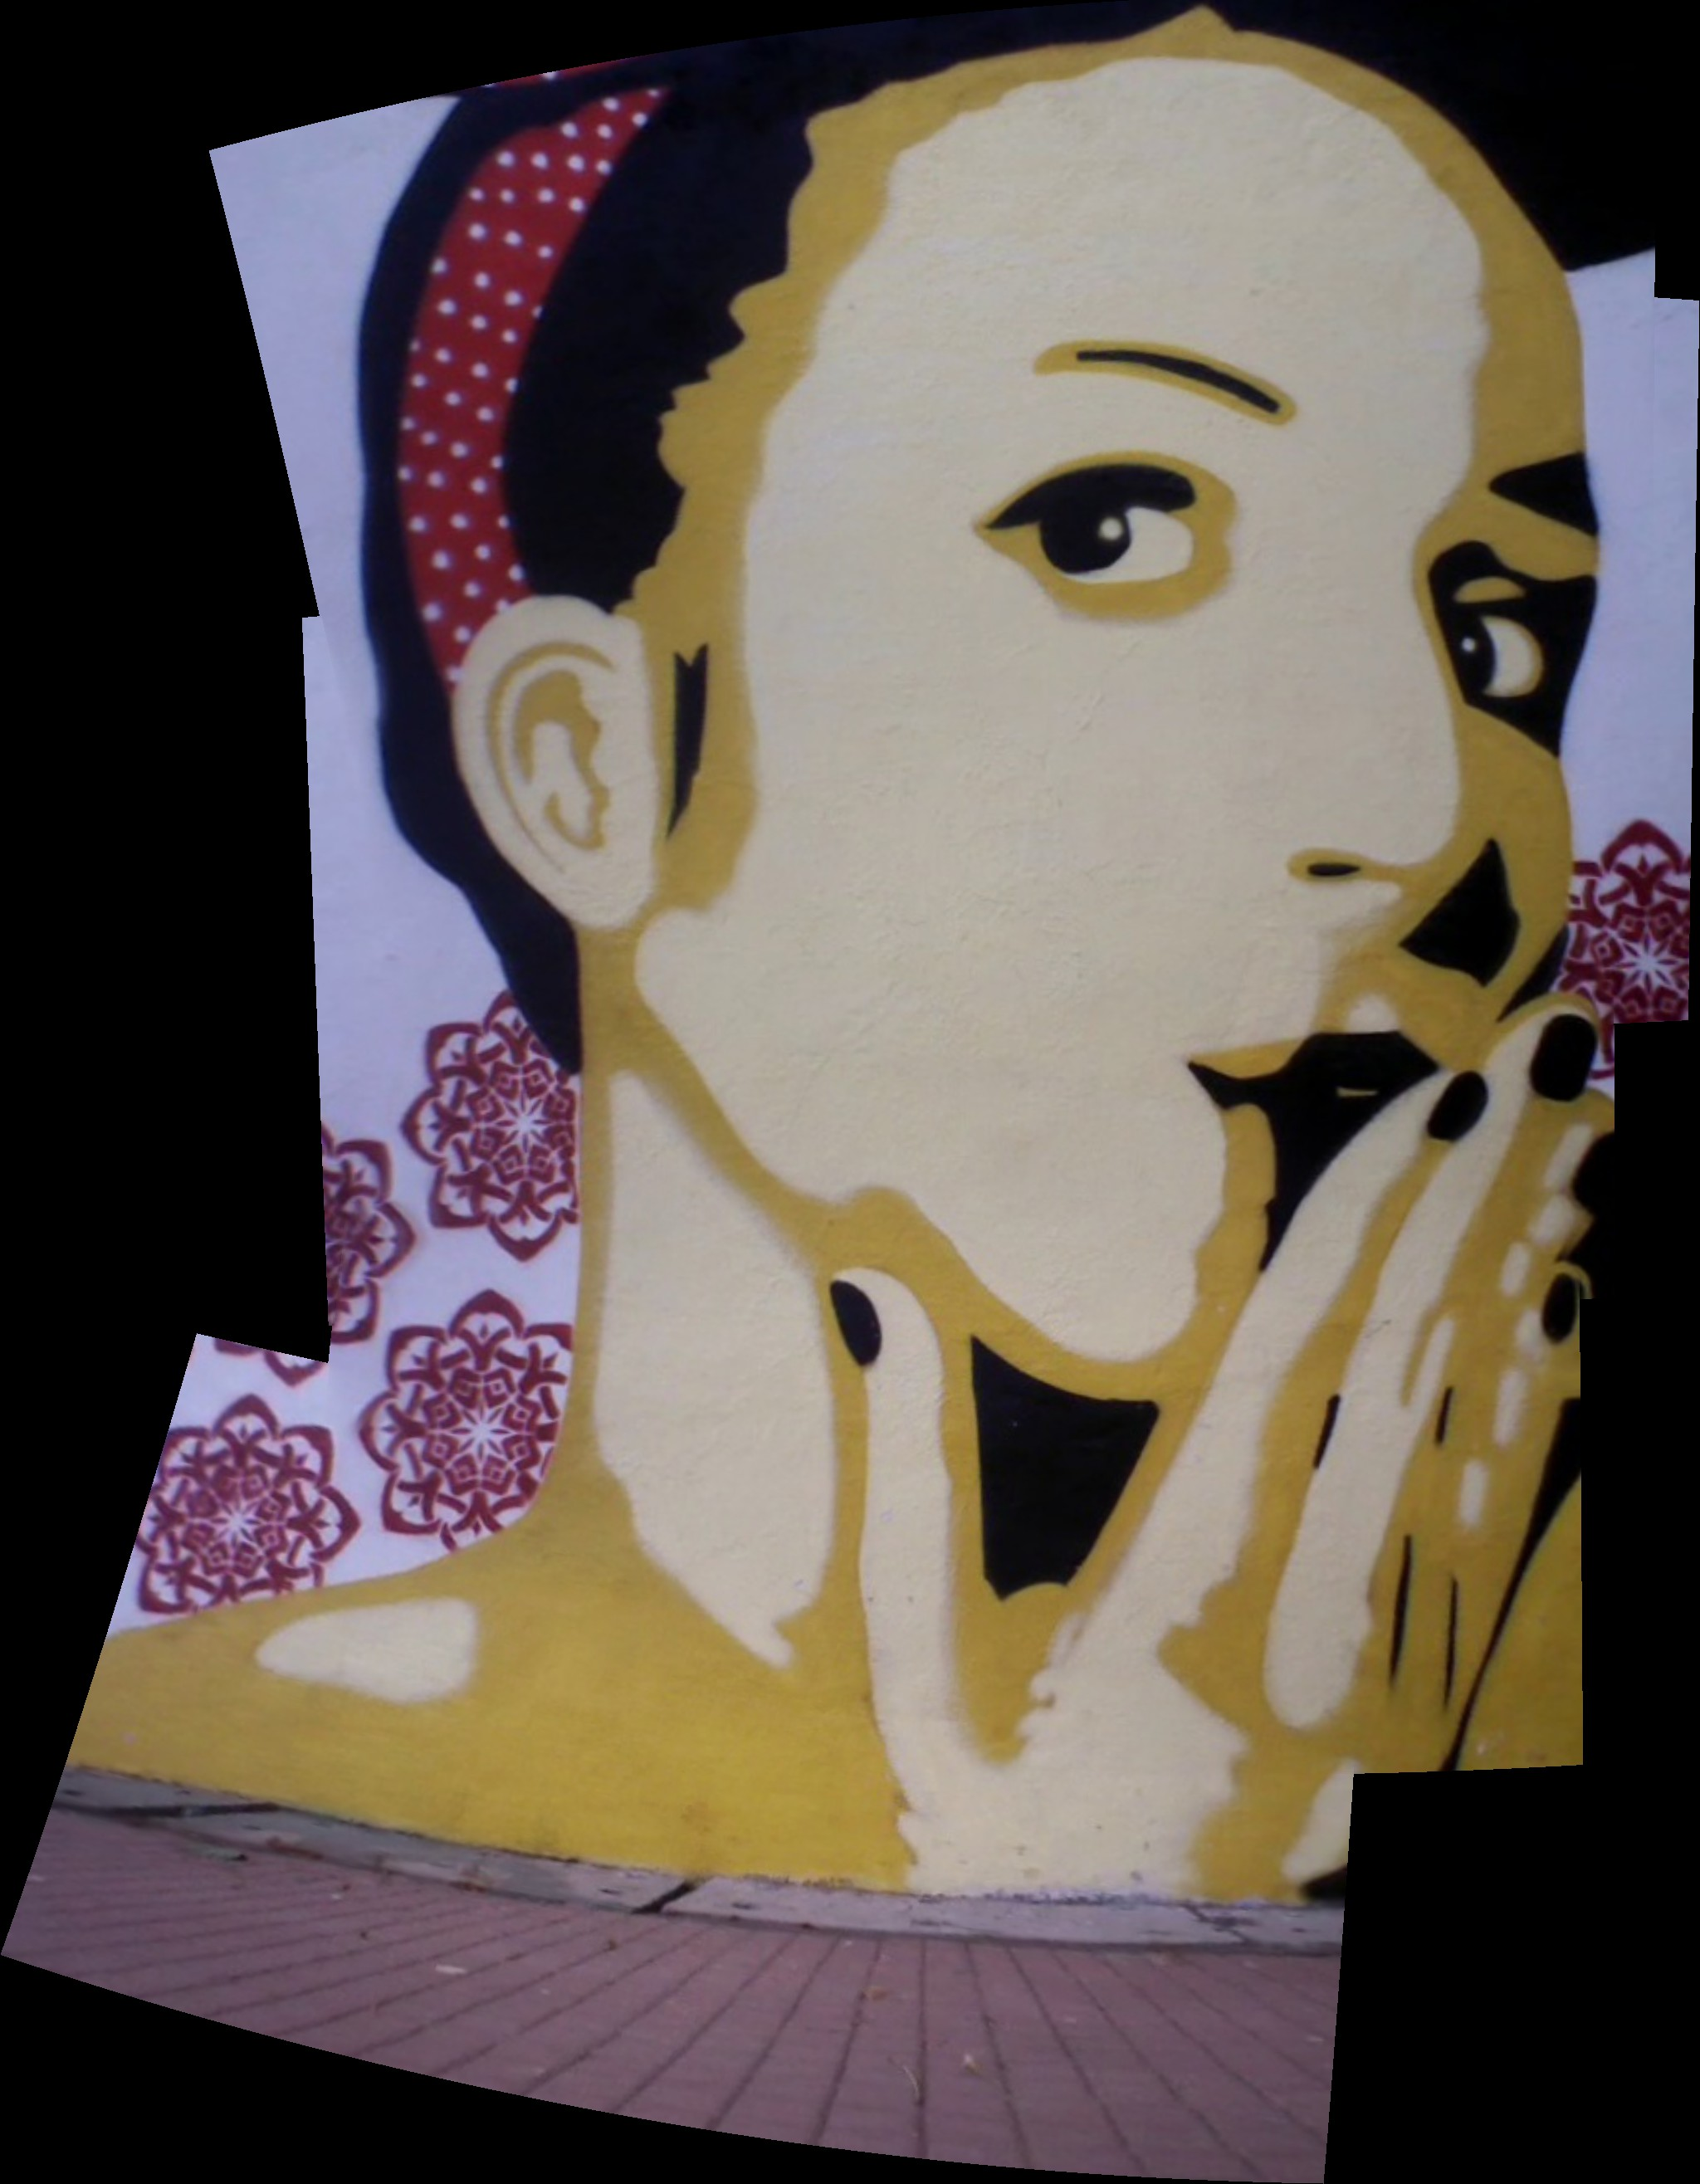
\includegraphics[width=\linewidth]{figures/sac3/autostitch.jpg}
\caption{Autostitch Result}
\end{subfigure}
\begin{subfigure}[b]{0.3\textwidth}
\centering
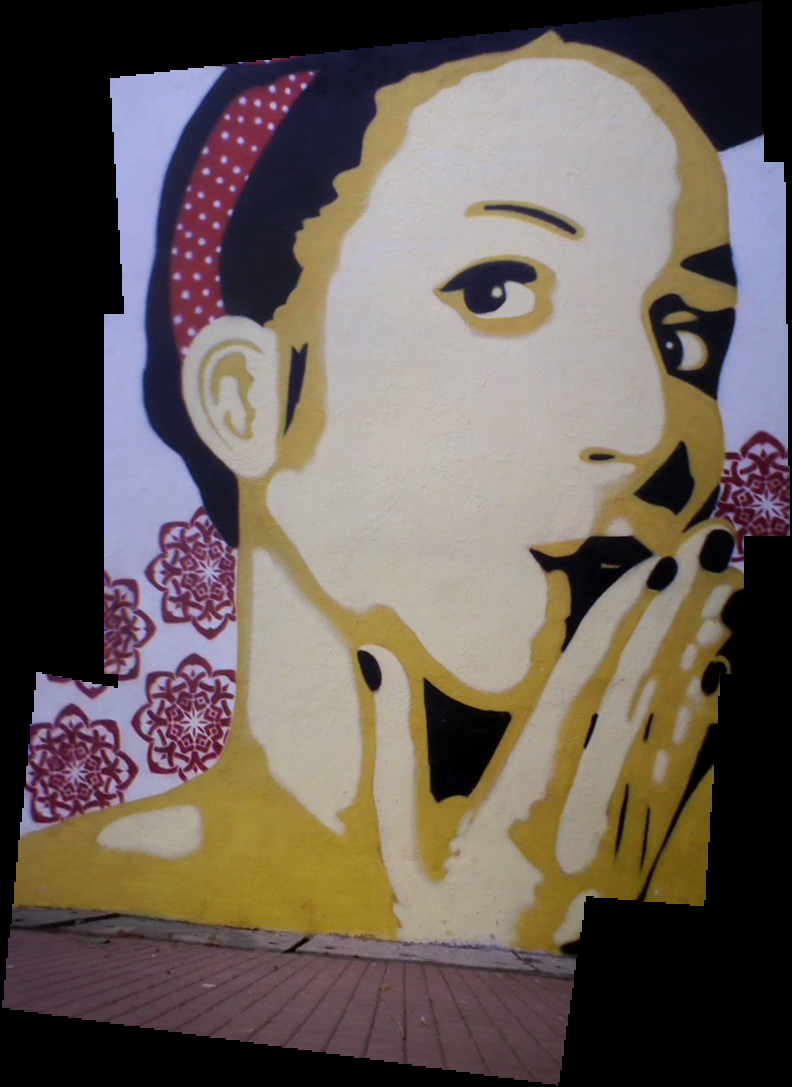
\includegraphics[width=\linewidth]{figures/sac3/photoshop.jpg}
\caption{Photoshop Result}
\end{subfigure}
\begin{subfigure}[b]{0.3\textwidth}
\centering
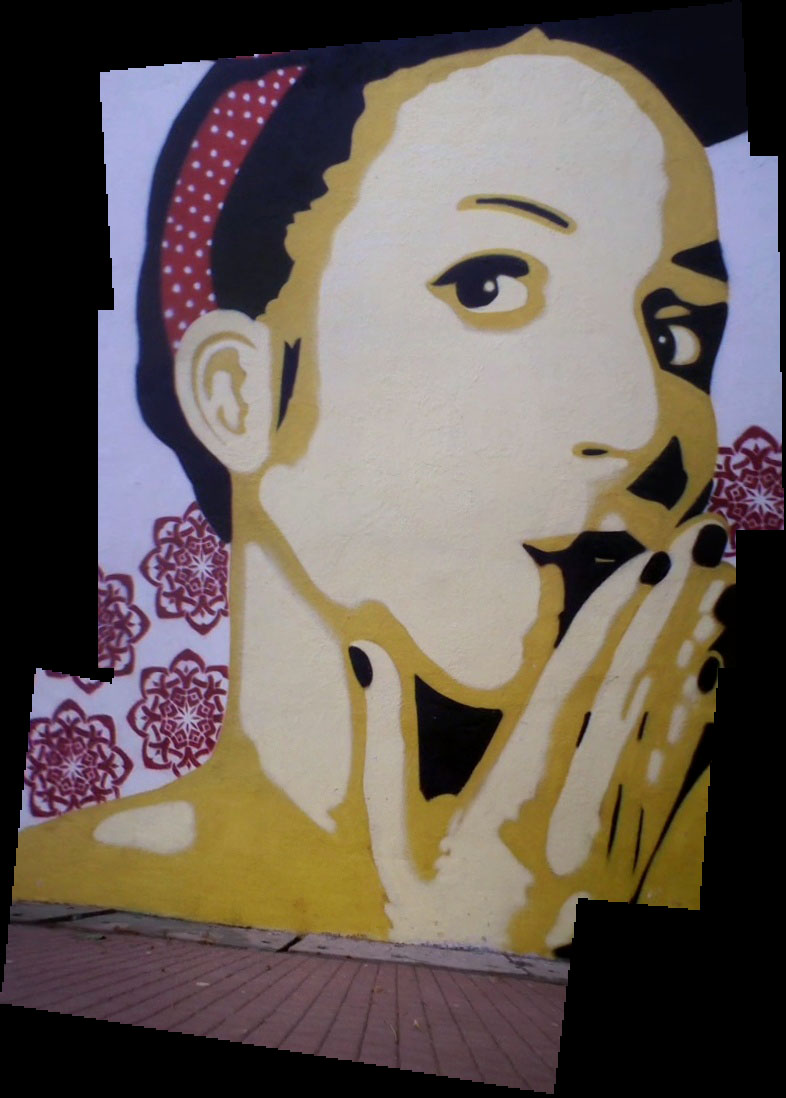
\includegraphics[width=\linewidth]{figures/sac3/our_result.jpg}
\caption{Our Result}
\end{subfigure}
\caption{Comparison of outputs of Autostich, Photoshop and our stitching
algorithm on the images selected by our algorithm. Our output is comparable
with output of Photoshop and Autostitch.}
\label{fig:results_sac3}
\end{figure*}

\subsection{Indoor Imagery with Dead Space} 

Our next selection of experiments were conducted in an indoor
environment with some natural light.  The input stream had about 4300
images. The selection algorithm pruned the video into N=4 images. A sample of the selected images are
seen in Figure \ref{fig:idc_selected}

\begin{figure}
\centering

\includegraphics[width=0.22\linewidth]{figures/idc_indoor/selected/1.jpg}

\includegraphics[width=0.22\linewidth]{figures/idc_indoor/selected/2.jpg}

\includegraphics[width=0.22\linewidth]{figures/idc_indoor/selected/3.jpg}

\includegraphics[width=0.22\linewidth]{figures/idc_indoor/selected/4.jpg}
\caption{Sample selected images of indoor scene by our algorithm.}
\label{fig:idc_selected}
\end{figure}

There were two disconnected components in the resulting graph. The ground truth
can be seen in Figure \ref{fig:idc_indoor_groundtruth}.

\begin{figure}
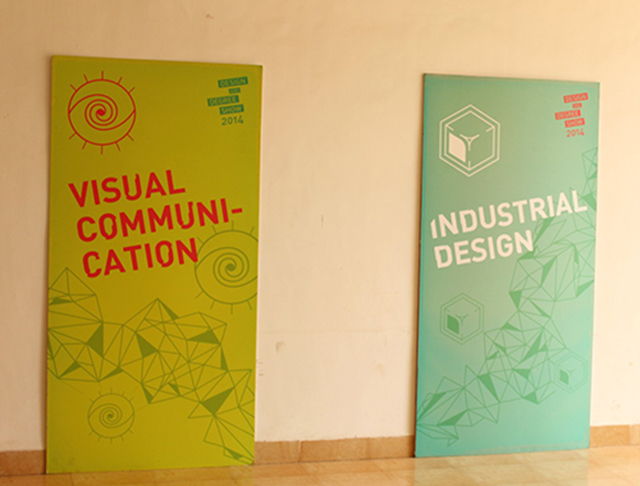
\includegraphics[width=\linewidth]{figures/idc_indoor/groundtruth.jpg}
\caption{Ground truth of the indoor scene captured by quadcopter. There is
visible gap in betwen two posters which will cause problems for state of the art
stitchers.}
\label{fig:idc_indoor_groundtruth}
\end{figure} 

Figure \

\begin{figure*}
\begin{subfigure}[b]{0.3\textwidth}

\includegraphics[width=\linewidth]{figures/idc_indoor/autostitch.jpg}
\caption{Autostitch Result}
\end{subfigure}
\begin{subfigure}[b]{0.3\textwidth}
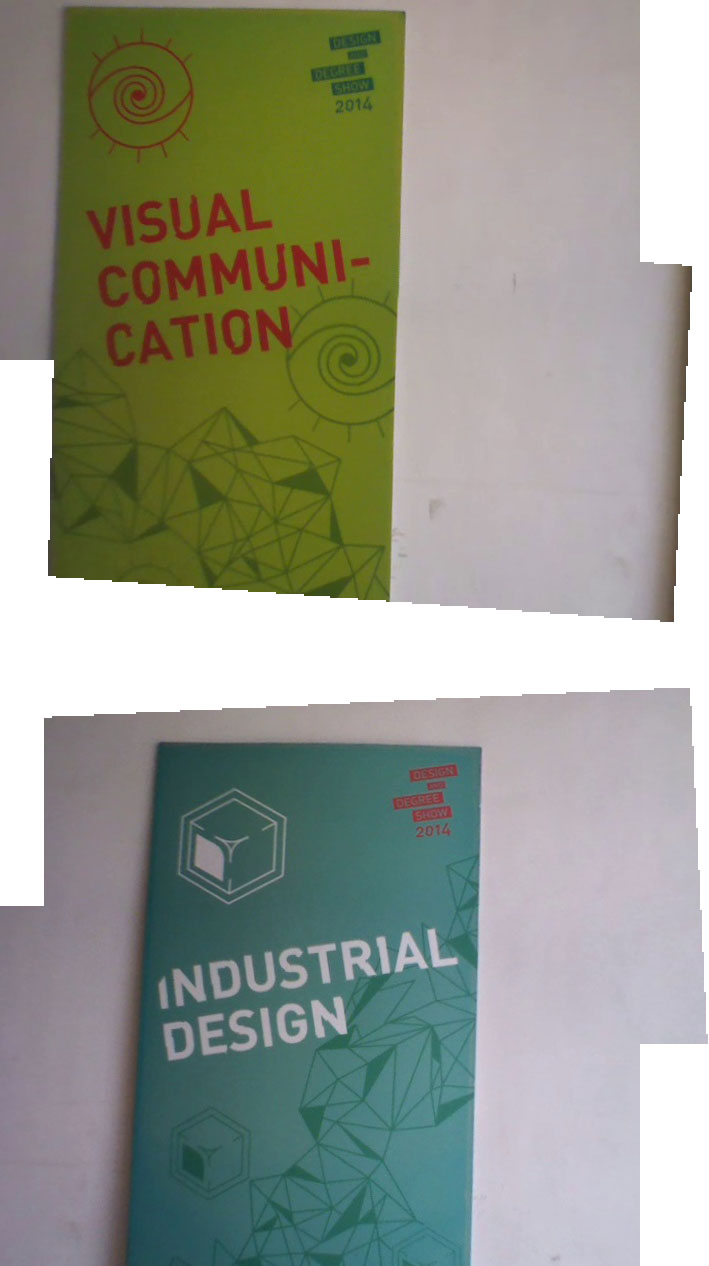
\includegraphics[width=\linewidth]{figures/idc_indoor/photoshop.jpg}
\caption{Photoshop Result}
\end{subfigure}
\begin{subfigure}[b]{0.3\textwidth}
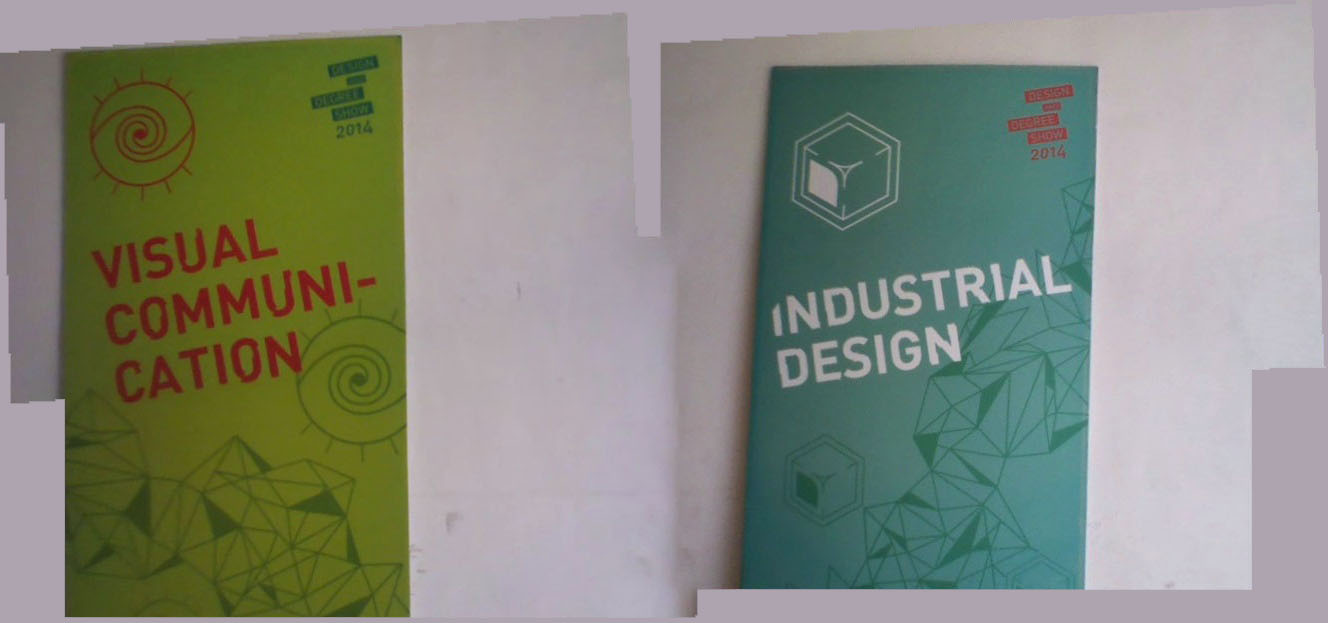
\includegraphics[width=\linewidth]{figures/idc_indoor/our_result.jpg}
\caption{Our Result}
\end{subfigure}
\caption{Comparison of outputs of Autostich, Photoshop and our stitching
algorithm on the images selected of indoor scene by our algorithm. Only our
output is able to shows individual panoramas at their respective location
approximately}
\label{fig:idc_indoor_comparison}
\end{figure*}

One can see a better orthographic view of the posters in a composite
manner. Autostitch was unable to produce any reasonable output as seen in
Figure \ref{fig:idc_indoor_comparison}.

\subsection{Outdoor Imagery with Dead Space}


